\documentclass[paper.tex]{subfiles}

\begin{document}


\section{Proof that $\mathcal{V}$ is a universal template}

In this section we outline the proof given in full detail in~\cite{Ghrist1996} that $\V$ (shown in Figure~\ref{fig:universal}) is a universal template. Details will inevitably be omitted but our goal in this exposition is to straddle the line between
the full proof and the very high-level outline given in~\cite{knottyode}, giving a concise and readable exposition that gets at the essence of the proof.

The essential idea is to find a special set of templates which have a special property that forces them to support all braids as orbits, and then to show that these templates can be found in $\V$. Since all knots and links
can be realized as a braid, this immediately implies that $\V$ is universal. The last step of showing that the special braid-supporting templates can found in $\V$ is the most difficult by far and where we will have to do the
most hand-waving. Nonetheless, we will try to capture the essence.

Also important in this proof is the existence of the $\mathcal{U}$ template, pictured below. $\mathcal{U}$ and $\V$ are essentially equivalent, but there is one minor difference, and $\mathcal{U}$ is universal as well.

\begin{figure}[h]
  % not sure where to put this, but not here

    %this doesn't seem like too bad of a spot; you mention figure 1 in the first paragraph of this section so it shouldn't be placed too far away from that paragraph
  \centering
  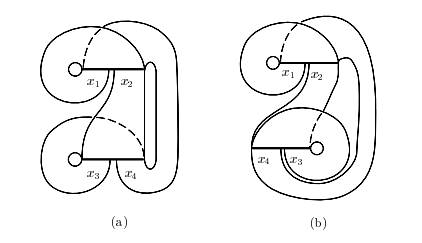
\includegraphics[width=0.8\textwidth]{universalVU.png}
  \caption{(a) The universal template $\V$ and (b) The universal template $\mathcal{U}$, reproduced from~\cite{ghs1997}}\label{fig:universal}
\end{figure}


\subsection{Braids and the theorem of Alexander}

Recall that a closed braid is a collection of $P$ disjoint simple closed curves in a standardly embedded torus $D^2 \times S^1$ such that every $D^2$ cross-section of the torus intersects the closed braid in exactly $P$ points.

% related to pure braid group/symmetric group -- this following line isn't entirely accurate, so I've commented it out for now
%Braids have a natural identification as a permutation on $P$ elements, which is the property we exploit.

In a landmark paper~\cite{Alexander1923}, Alexander proved the following theorem which provides the crucial connection
between braids and links.

% we exploit it since each permutation can be written as the product of exchanges

\begin{thm}[Alexander 1923]
  Each knot or link is isotopic to some closed braid on $P$ strands for some $P$
\end{thm}

\subsection{The templates $\W_q$}

The family of templates $\set{\W_q}$ shown in Figure~\ref{fig:w_q} are those referred to earlier as the braid-supporting templates. $\W_1$ is identically $\V$ and increasing $q$ by one has the effect of adding
two \emph{ears} of alternating `sign' to one side. The property that successive ears alternate in `sign' is what makes this family of templates so useful, as this property makes proving that they support all braids delightfully simple.

\begin{figure}[h]
  \centering
  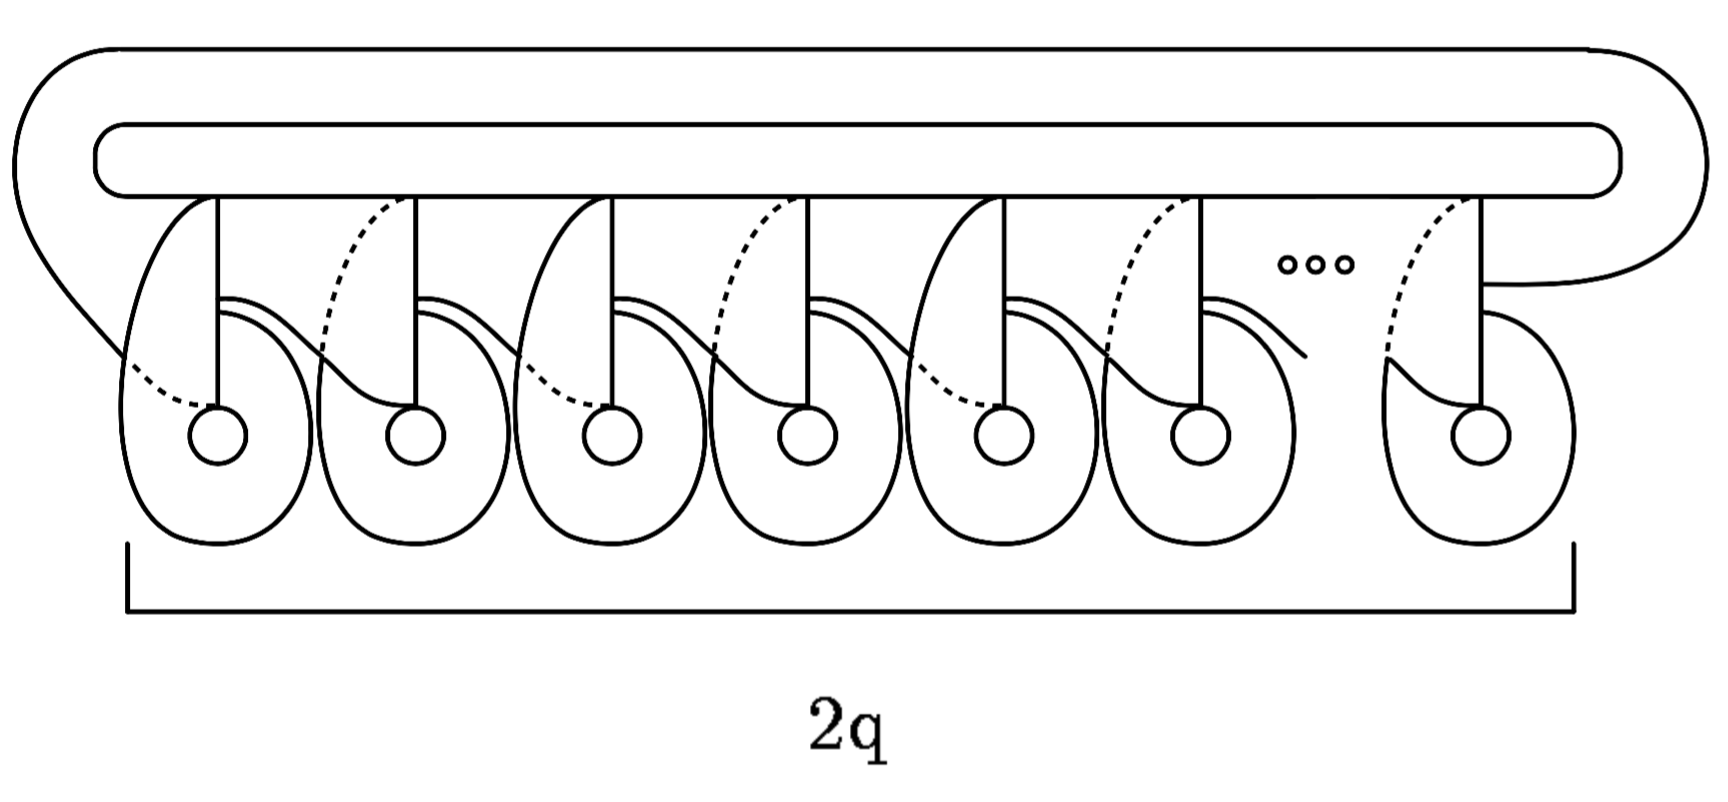
\includegraphics[width=0.8\textwidth]{w_q.png}
  \caption{The templates $W_q$, reproduced from~\cite{knottyode}}\label{fig:w_q}
\end{figure}


\begin{lemma}[Ghrist 1996]
  An isotopic copy of any closed braid exists as a set of periodic orbits on some $W_q$ for sufficently large $q$.
\end{lemma}

\begin{proof}

    The concatenation of alternating positive and negative ears on $\W_q$ mimics the braid group concatenation operation. The braid group $B_{n+1}$ is naturally generated by $\sigma_1, \sigma_2, \dots, \sigma_{n}$, where $\sigma_i$ is a single crossing of the $i$th strand over the $(i + 1)$th strand and its inverse, $\sigma_i^{-1}$, is a single crossing of the $(i + 1)$th strand over the $i$th strand. Naturally, $\sigma_i \sigma_i^{-1} = \sigma_i^{-1} \sigma_i = I$. We can consider the elements $\pi_1, \pi_2, \dots, \pi_n, \pi_1', \pi_2', \dots, \pi_n'$ of $B_{n+1}$, where $\pi_i = \sigma_1 \sigma_2 \cdots \sigma_i$ and $\pi_i' = \sigma_1^{-1} \sigma_2^{-1} \cdots \sigma_i^{-1}$. Note that $\pi_1 = \sigma_1$, $\pi_1' = \sigma_1^{-1}$, and that for $i > 1$,

    \begin{align*}
        \pi_{i-1}^{-1} \pi_i  &= (\sigma_1 \sigma_2 \dots \sigma_{i - 1})^{-1} \sigma_1 \sigma_2 \cdots \sigma_i \\
                              &= \sigma_{i - 1}^{-1} \cdots \sigma_2^{-1} \sigma_1^{-1} \sigma_1 \sigma_2 \cdots \sigma_i \\
                              &= \sigma_{i - 1}^{-1} \cdots \sigma_2^{-1} \sigma_2 \cdots \sigma_i \\
                              &= \sigma_{i - 1}^{-1} \sigma_{i - 1} \sigma_i  \\
                              &= \sigma_i \\ \\
        \pi_{i-1}'^{-1} \pi_i'  &= (\sigma_1^{-1} \sigma_2^{-1} \dots \sigma_{i - 1}^{-1})^{-1} \sigma_1^{-1} \sigma_2^{-1} \cdots \sigma_i^{-1} \\
                                &= \sigma_{i - 1} \cdots \sigma_2 \sigma_1 \sigma_1^{-1} \sigma_2^{-1} \cdots \sigma_i^{-1} \\
                                &= \sigma_{i - 1} \cdots \sigma_2 \sigma_2^{-1} \cdots \sigma_i^{-1} \\
                                &= \sigma_{i - 1} \sigma_{i - 1}^{-1} \sigma_i^{-1}  \\
                                &= \sigma_i^{-1} \\ \\
    \end{align*}

    We can conclude that the elements $\pi_1, \pi_2, \dots, \pi_n, \pi_1', \pi_2', \dots, \pi_n'$ of $B_{n+1}$ are a generating set for $B_{n+1}$.

    %it's possible to split this proof into two, one half for proving the above is a generating set for B_{n+1} and second half for concluding that W_q contains all braids for large q

    For the braid group $B_{n+1}$, notice that for all $1 \leq i \leq n$, $\pi_i$ can be drawn on any positive ear of $\W_q$, letting all but the bottom strand take the top strip and forcing the bottom strand to take the bottom strip, cross over exactly $i$ strands, and take the top strip. Similarly, for all $i \leq i \leq n$, $\pi_i'$ can be drawn on any negative ear of $W_q$, letting all but the bottom strand take the top strip, forcing the bottom strand to take the bottom strip, cross under exactly $i$ strands, and take the top strip. Examples of $\pi_2$ and $\pi_2'$ of the braid group $B_5$ are drawn in Figure~\ref{fig:earexchange}.

    Because this set of elements generates the braid group $B_{n+1}$, any braid $B \in B_{n+1}$ can be drawn as a sequence of $\pi_i$ and $\pi_i'$. If $B$ can be represented with $m$ of these elements, then the closure of $B$ lies in $W_m$, as $W_m$ contains $m$ pairs of positive/negative ears that can each support a $\pi_i$ or $\pi_i'$ structure. Thus, any closed braid on $N$ strands lies in $W_q$ for sufficiently large $q$.

\end{proof}



\begin{figure}[h]
  \centering
  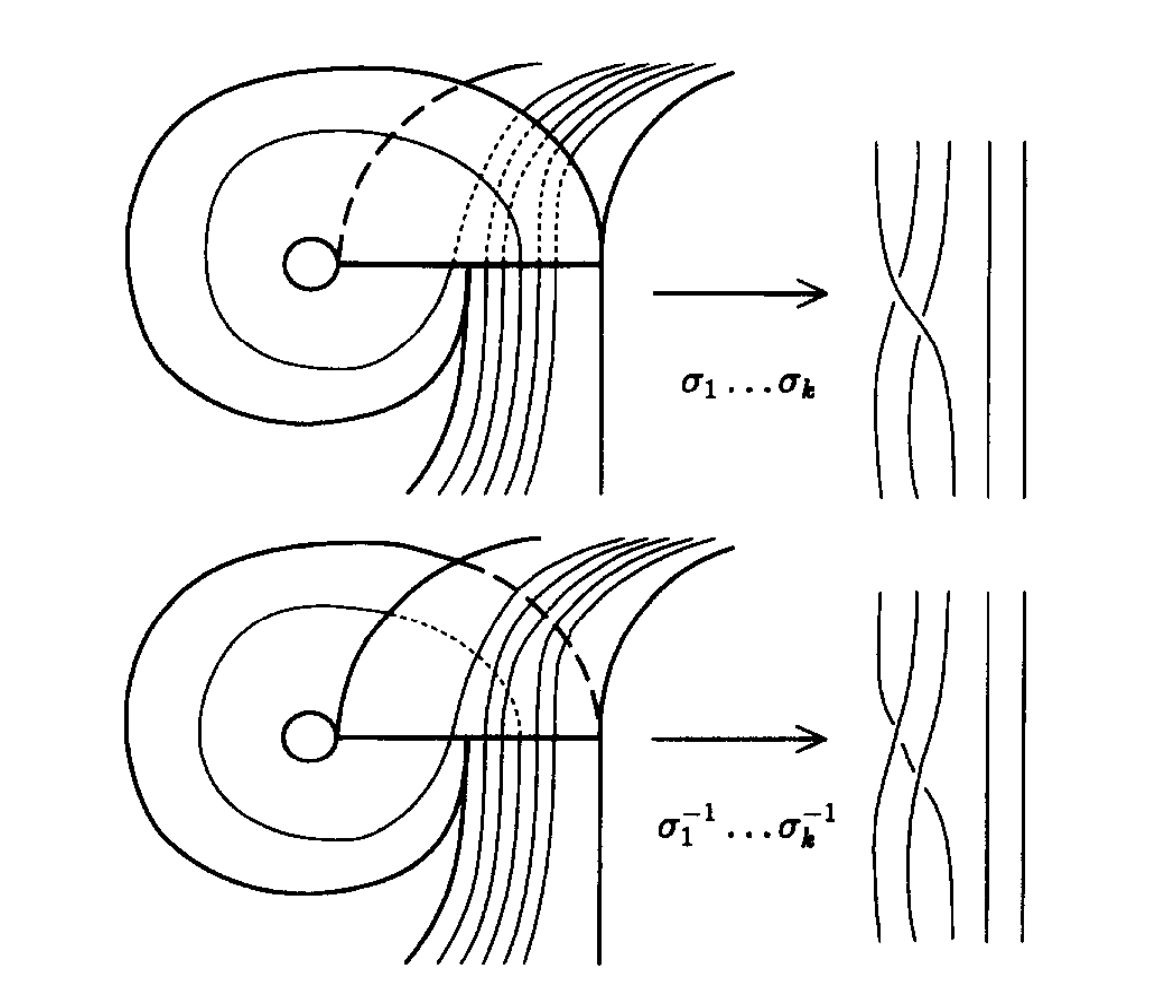
\includegraphics[width=0.8\textwidth]{ear_exchange.png}
  \caption{Top: $\pi_2$ in $B_5$ Bottom: $\pi_2'$ in $B_5$. Figure reproduced from~\cite{Ghrist1996}}\label{fig:earexchange}
\end{figure}




%\subsection{Construct $\W_{q+1}$ from $\W_q$}

%Start with renormalized $\W_1 \in \V$, and append a pair of ears to\dots

% is this actually necessary?


\subsection{Special Inflations: $\mathcal{F}$ and $\mathcal{G}$}

In his proof, Ghrist uses a few special inflations, $\mathcal{F}$ and $\mathcal{G}$, and accompanies them with a proposition:

\begin{prop}
    The following inflations are isotopic.
$$F: U \hookrightarrow \V \begin{cases} x_1 \mapsto x_1 \\ x_2 \mapsto x_1 x_2 x_3 \\ x_3 \mapsto x_4 x_2 \\ x_4 \mapsto x_4 \end{cases}$$

$$G: \V \hookrightarrow U \begin{cases} x_1 \mapsto x_1 \\ x_2 \mapsto x_1 \\ x_3 \mapsto x_2 x_4 \\ x_4 \mapsto x_2 x_3 x_4 \end{cases}$$
\end{prop}

As proof of their isotopy, diagrams showing the inflation are given.


\begin{figure}[h]
  \centering
  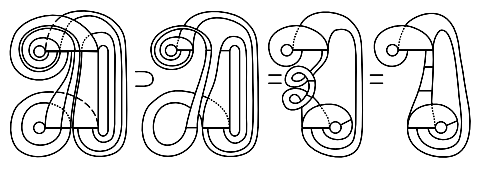
\includegraphics[width=0.8\textwidth]{inflationF.png}
  \caption{Left to Right: A subtemplate of $\V$ as given by $\mathcal{F}$, then cut along the boundary and removed from $\V$, simplified to show that it equals $\mathcal{U}$. Figure reproduced from~\cite{ghs1997}}\label{fig:isotopicF}
\end{figure}

\begin{figure}[h]
  \centering
  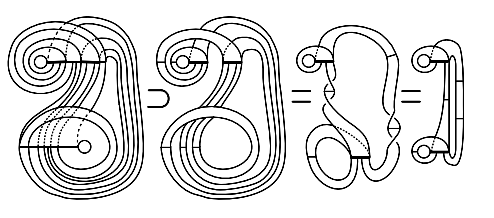
\includegraphics[width=0.8\textwidth]{inflationG.png}
  \caption{Left to Right: A subtemplate of $\mathcal{U}$ as given by $\mathcal{G}$, then cut along the boundary and removed from $\mathcal{U}$, simplified to show that it equals $\V$. Figure reproduced from~\cite{ghs1997}}\label{fig:isotopicG}
\end{figure}


In addition, we can consider the following inflation: $$\chi: \begin{matrix} U \mapsto U \\ \V \mapsto \V \end{matrix} \begin{cases} x_1 \mapsto x_3 \\ x_2 \mapsto x_4 \\ x_3 \mapsto x_1 \\ x_4 \mapsto x_2 \end{cases}$$

    The purpose of this inflation is to switch the two branch lines.

    \begin{lemma}[Ghrist 1997]
        Given an isotopic inflation $A$ having either $\mathcal{U}$ or $\V$ as a domain and range (independently of each other), the inflation $A^* = \chi A \chi$ is also isotopic.
    \end{lemma}

For example, given $\mathcal{F}$ as defined above, $mathcal{F}^*$ is defined as $$mathcal{F}^*: U \hookrightarrow \V \begin{cases} x_1 \mapsto x_2 x_4 \\ x_2 \mapsto x_2 \\ x_3 \mapsto x_3 \\ x_4 \mapsto x_3 x_4 x_1 \end{cases}$$ Because $\mathcal{F}$ is isotopic, we know that $mathcal{F}^*$ must be isotopic as well; in addition, $mathcal{G}^*$ is also isotopic.

    Finally, in the next section, we can include the inflation $\mathfrak{H} = mathcal{F}^* G F mathcal{G}^*$ in the next section to continue our proof.


\subsection{Find $\W_q \subset \V$ for all $q$}

We must start with a lemma, provided by Ghrist.
\begin{lemma}[Ghrist 1997]
    Given that a subtemplate of $\V$ doesn't contain $x_1^\infty$, it is possible to add an ear near the top branch line, like that in Figure~\ref{fig:appendToV}, which is a positive ear. Similarly, given that a subtemplate of $\V$ doesn't contain $X_3^\infty$, it is possible to add an ear near the bottom branch line, which is a negative ear.
\end{lemma}


Now, we prove that $\W_q \subset \V$ for all $q$.

\begin{proof}
Let us begin with $\W_1 = \V$. We calculate the inflation $\mathfrak{H} = mathcal{F}^* G F mathcal{G}^*$. This is done by taking $x_1$ in $mathcal{G}^*$ to be $x_4 x_2$, then substituting those values of $x_4$ and $x_2$ in $\mathcal{F}$ to get $x_4 x_1 x_2 x_3$. Each of these is found in $\mathcal{G}$ and substituted to get $x_2 x_3 x_4 x_1^2 x_2 x_4$, then lastly we find these in $mathcal{F}^*$ to get what $x_1$ is finally mapped to. We can do the same for the other strips.
    $$\mathfrak{H}: \V \hookrightarrow \V \begin{cases}
        x_1 \mapsto x_2 x_3^2 x_4 x_1 (x_2 x_4)^2 x_2 x_3 x_4 x_1 \\
        x_2 \mapsto x_2 x_3^2 x_4 x_1 (x_2 x_4)^3 x_2 x_3 x_4 x_1 \\
        x_3 \mapsto x_2 x_3^2 x_4 x_1  x_2 x_4  \\
        x_4 \mapsto x_2 x_3^2 x_4 x_1  x_2 x_4  \end{cases} $$

        Note that $mathcal{G}^*$ is an isotopic inflation from $\V$ to $\mathcal{U}$, $\mathcal{F}$ is an isotopic inflation from $\mathcal{U}$ to $\V$, $\mathcal{G}$ is an isotopic inflation from $\V$ to $\mathcal{U}$, and that $mathcal{F}^*$ is an isotopic inflation from $\mathcal{U}$ to $\V$. It must follow that $\mathfrak{H}$ is an isotopic inflation from $V$ to $V$; in other words, an isotopic renormalization.

        This renormalization satisfies the condition that this subtemplate does not contain $x_1^\infty$. Then, after performing this renormalization, we will be able to add a positive ear at the top branch line; after doing so, we now have $\W_1^+$.

        There exists a very similar inflation $\mathfrak{H}^*$ from $\V$ onto $\V$ that will allow us to add a negative ear at the bottom branch line. Now, we have added a positive ear and a negative ear, so we are at $\W_2$, yet this subtemplate is still contained within $\V$; this implies that $\W_2 \subset \V$. Now, we can repeat this procedure, adding another positive and negative ear after the respective inflations to get $\W_3$.

        This procedure can be repeated $q$ times to show that $\W_q \subset \V$ for any positive $q$; thus, by induction, $\W_q \subset \V$ for all $q$.
    \end{proof}


\begin{figure}[h]
    \centering
    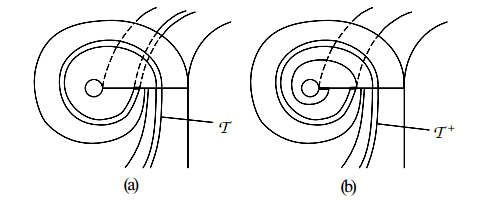
\includegraphics[width=0.8\textwidth]{appendToV.png}
    \caption{Appending a positive ear to $T$ (left) yields $T^+$ (right). Figure reproduced from~\cite{Ghrist1996}} \label{fig:appendToV} %%%%%%%%%%%%%%%%%%%%% link below.
\end{figure}



\subsection{Universal Templates and V}

\begin{thm}[Ghrist 1996]
    The template $\V$ contains an isotopic copy of every tame knot and link as a periodic orbit of the semiflow.
\end{thm}
\begin{proof}
    This proof comes immediately following the fact that $\W_q \subset \V$ for all $q$, and that all closed braids (and thus all tame links and knots) can be contained within $\W_q$ for large enough $q$. Thus, $\V$ contains every tame knot and link.
\end{proof}


Ghrist then extends the theorem above to prove the following:

\begin{thm}[Ghrist 1996]
    The template $\V$ contains all orientable templates as subtemplates of $\V$.
\end{thm}

It must follow that if there are any other universal templates $T$, then $\V$ must contain $T$ as a subtemplate. As $T$ contains all tame links and knots as well, as it is universal, the same theorems can be applied to $T$ as were applied to $\V$, so that $T$ also contains all templates (including $\V$).



\end{document}
